30. \begin{figure}[ht!]
\center{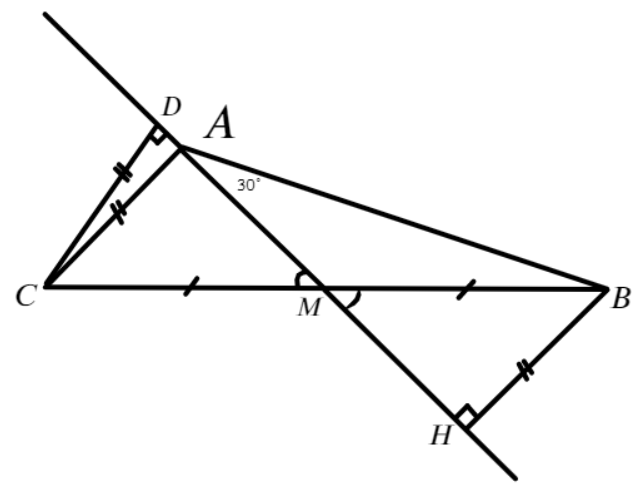
\includegraphics[scale=0.35]{g30.png}}
\end{figure}\\
Сделаем дополнительное построение: опустим из точки $B$ перпендикуляр $BH$ на продолжение медианы $AM.$ Треугольник $ABH$ является прямоугольным и катет $BH$ лежит напротив угла в $30^\circ,$ поэтому $BH=\frac{1}{2}AB=AC.$ Теперь опустим перпендикуляр $CD$ из точки $C$ на прямую $AM.$ Углы $DMC$ и $HMB$ являются вертикальными, $CM=MB$ (так как $AM$ медиана), значит прямоугольные треугольники $DMC$ и $HMB$ равны по гипотенузе и острому углу, поэтому $CD=BH=AC.$ Но тогда в прямоугольном треугольнике $CDA$ катет равен гипотенузе, что невозможно, значит точка $D$ совпадает с точкой $A$ и $\angle CAM=90^\circ.$ Таким образом, $\angle BAC=90^\circ+30^\circ=120^\circ.$
ewpage

oindent31. \begin{figure}[ht!]
\center{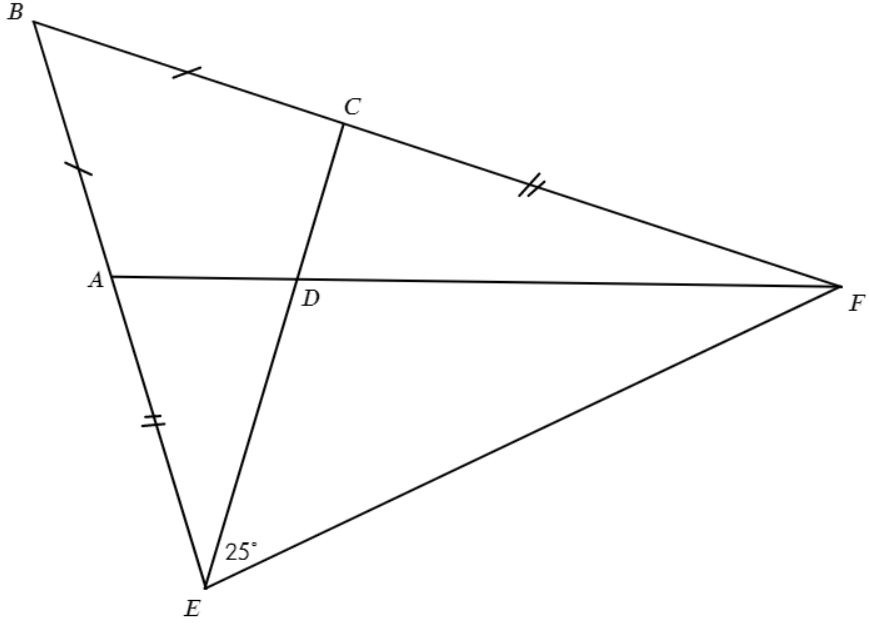
\includegraphics[scale=0.35]{g31.png}}
\end{figure}\\
Заметим, что $AE=BE-AB=BF-BC=CF.$ Треугольник $EBF$ является равнобедренным $(BE=BF),$ значит $\angle BEF=\angle BFE.$ Тогда
$\left.\begin{array}{l}AE=CF,\\
\angle AEF=\angle CFE,\\
EF\text{--- общая.}  \end{array}
ight\}\Rightarrow \Delta AEF=\Delta CFE\text{ по I призн.}$\\$\Rightarrow \angle EFD=\angle EFA=\angle CEF=\angle DEF=25^\circ.$\\
